\section{Theorie}
\label{sec:Theorie}


\subsection{Fehlerrechnung}

Für die Fehlerfortpflanzung bei Gleichungen mit $N$ fehlerbehafteten Größen
wird jeweils die Formel zur Gaußschen Fehlerfortpflanzung

\begin{equation}
  \sigma = \sqrt{\sum_{i=1}^{N}\biggl(\frac{\partial f(x_i)}{\partial x_i}
  \sigma_i\biggr)^2}
\end{equation}
mit der jeweiligen Funktion $f(x_i)$, den Messgrößen $x_i$ und den
zugehörigen Fehlern $\sigma_i$ verwendet.
Zur Berechnung des arithmetischen Mittels von $N$ Messwerten wird jeweils die
Formel

\begin{equation}
  \bar{x} = \frac{1}{N}\sum_{i=1}^{N}x_i
\end{equation}
mit den Messwerten $x_i$ benutzt.
die Standardabweichung des Mittelwerts wird jeweils mit der Gleichung

\begin{equation}
  \bar{\sigma} = \sqrt{\frac{1}{N-1}\sum_{i=1}^{N}(x_i - \bar{x})^2}
\end{equation}
mit den $N$ Messwerten $x_i$ berechnet.


\subsection{Problemstellung}

In der Mechanik unterscheidet man bei externen Kräften auf Körper zwischen
solchen, die an Volumenelementen angreifen und somit den gesamten Körper
bewegen können, und solchen, die an Oberflächenelementen angreifen und somit
den Körper deformieren können.
Da die Oberflächenkräfte auf Ober- und Querschnittsflächen eines Körpers wirken,
wird die Spannung, das ist der Quotient aus Kraft und Flächenelement,
eingeführt.
Es wird zwischen dem Druck $P$, also der Spannung, die senkrecht auf der
Oberfläche steht, und der Tangentialspannung $\tau$, die parallel zur Oberfläche
steht, unterschieden.
Im folgenden Versuch wird eine elastische Deformation, das ist eine
Deformation, bei der sich ein Körper nach einer Belastung wieder zurückverformt,
durch Tangentialspannungen an einem Probekörper untersucht.


\subsection{Hookesches Gesetz}

Die Proportionalität zwischen Spannung und Volumenänderung
$\frac{\Delta V}{V}$ oder
Längenänderung $\frac{\Delta L}{L}$ bei hinreichend geringen Spannungen
wird im Hookeschen Gesetz

\begin{align}
  v & = \alpha \frac{\Delta V}{V} & l & = \beta \frac{\Delta L}{L} \\
  \label{eqn:Hooke}
\end{align}
zusammengefasst.
die Abstände zwischen den Molekülen und Atomen eines Körpers bleiben ohne
äußere Einwirkung durch elektrostatische Kräfte im Gleichgewicht $r_0$.
Wird der Köper unter Spannung gesetzt und deformiert, so verändern sich die
Abstände zu $r'_0$.
Bis zu einem bestimmten Abstand, der abhängig vom Körper ist, ist die
Deformation elastisch.
In Abbildung \ref{fig:HookBe} ist der sogenannte Hookesche Bereich, der zwischen
diesem Abstand und der Gleichgewichtslage $r_0$ liegt, dargestellt.

\begin{figure}[h]
  \centering
  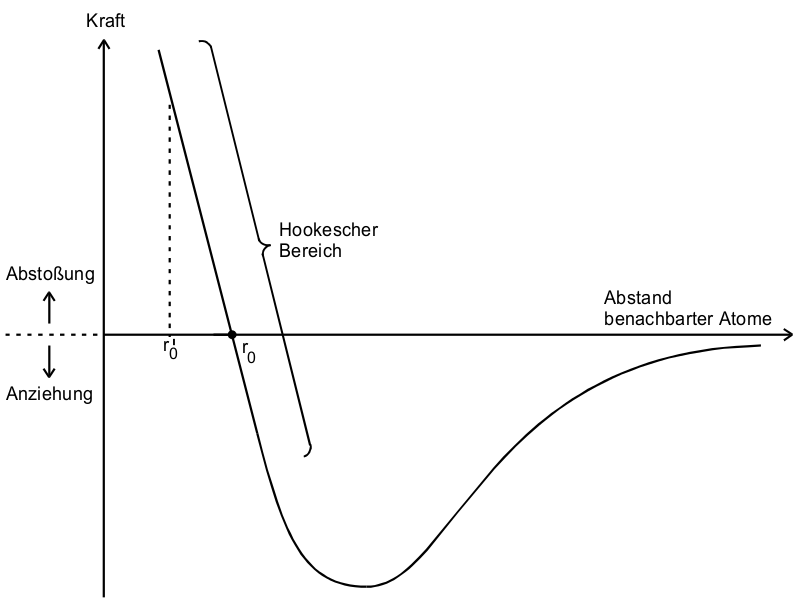
\includegraphics[height = 9cm]{HookescherBereich.png}
  \caption{Anziehung und Abstoßung benachbarter Atome nach Veränderung des
  Abstandes aus der Gleichgewichtslage $r_0$.}
  \label{fig:HookBe}
\end{figure}


\subsection{Elastische Konstanten}

Mit Hilfe der elastischen Konstanten kann der Zusammenhang zwischen
Deformation und Spannung an einem Körper vollständig beschrieben werden.
Werden Kristallgitter mit niedriger Symmetrie betrachtet, so besitzen sowohl
Spannung als auch Deformation jeweils sechs Freiheitsgerade, mit jeweils
drei, die die Gestalt beschreiben, und drei, die das Volumen beschreiben.
Der Zusammenhang wird über eine symmetrische 6x6-Matrix dargestellt,
weshalb insgesamt $21$ elastische Konstanten benötigt werden.
Im folgenden Experiment werden isotrope Materialien, das sind Stoffe deren
elastische Konstanten richtungsabhängig sind, benutzt.
Bei diesen Stoffen können Symmetrieeigenschaften so ausgenutzt werden,
dass sich das elastische Verhalten vollständig mit nur zwei Konstanten
beschreiben lässt.
Diese sind zum einen der Torsionsmodul $G$, der die
Gestaltselastizität beschreibt, und
der Kompressionsmodul $Q$, der die Volumenelastizität beschreibt.
Aus diesen Konstanten können zudem noch der Elastizitätsmodul $E$, der die
Längenanderung eines Körpers unter Einwirkung eines Drucks $P$ in Richtung
der Kraftwirkung beschreibt, und die Poissonsche Querkontraktionszahl $\mu$,
die die Längenanderung eines Körpers unter Einwirkung eines Drucks $P$
orthogonal zur Kraftwirkung beschreibt, bestimmt werden.
Letztere berechet sich mit der Formel

\begin{equation}
  \mu = - \frac{\Delta B}{B} \frac{L}{\Delta L}.
  \label{eqn:Querkontraktionszahl}
\end{equation}
Die Größen sind in Abbildung \ref{fig:Querkontra} dargestellt.

\begin{figure}
  \centering
  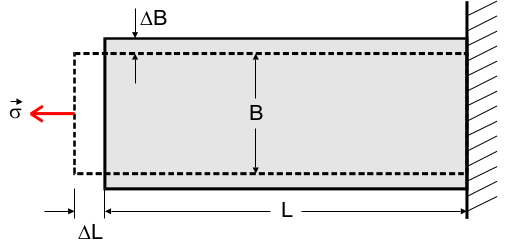
\includegraphics[height=4cm]{Querkontraktion.png}
  \caption{Erklärung der Querkontaktionzahl $\mu$ an einem gedehnten Stab.}
  \label{fig:Querkontra}
\end{figure}

Zwischen den vier Konstanten $\mu$, $E$, $Q$
und $G$ gelten die Beziehungen

\begin{align}
  E & = 2G(\mu + 1) \\
  E & = 3(1 - 2\mu)Q.
\end{align}


\subsection{Experimentelle Bestimmung elastischer Konstanten}

Von den vier erwähnten Konstanten eignet sich zur experimentellen Bestimmung
der Torsionsmodul $G$ am besten.
Eine mögliche Fehlerquelle bei der mehrfachen Messung des Moduls an einem
Körper ist die elastische Nachwirkung. Diese kann man vor Allem bei Metallen
beobachten. Das verformte Material kehrt nicht unmittelbar nach dem Ende der
Belastung in den Anfangszustand zurück, sondern in einem längeren Zeitraum.
Deshalb eignet sich zur Messung der Konstante eine sogenannte dynamische
Messreihe. Hierbei wird die Probe periodisch unter Spannung gesetzt, sodass
eine Rückverformung erzwungen wird.


\subsubsection{Bestimmung des Torsionsmoduls}

Prinzipiell kann das Torsionsmodul $G$ über den Winkel eines
durch eine angreifende Tangentialspannung $\tau$ verformten Würfels
wie in Abbildung \ref{fig:WurfelScher} bestimmt werden.

\newpage

\begin{figure}[h]
  \centering
  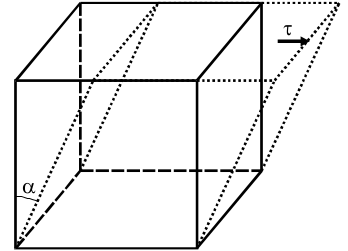
\includegraphics[height=4.5cm]{ScherungWuerfel.png}
  \caption{Scherung eines Würfels durch eine Tangentialspannung $\tau$.}
  \label{fig:WurfelScher}
\end{figure}

Die zur Grundfläche parallelen Flächen bleiben bei der Deformation quatratisch
und die gesuchte Konstante $G$ kann über den Scherungswinkel $\alpha$ mit der
Proportionalitätsformel

\begin{equation}
  \tau = \alpha G
  \label{eqn:Scherung}
\end{equation}
bestimmt werden.
Diese Messmethode eignet sich aber eher schlecht, da $\alpha$ nicht zuverlässig
bestimmt werden kann.
Hingegen eignet sich eine Messmethode, bei der ein Draht gedrillt
wird, deutlich besser. Hier für spannt man, wie in Abbildung \ref{fig:Torsion}
abgebildet, einen Draht an einer Seite fest und setzt ihn an der anderen Seite
an zwei diametralen Punkten unter Tangentialspannung.

\begin{figure}
  \centering
  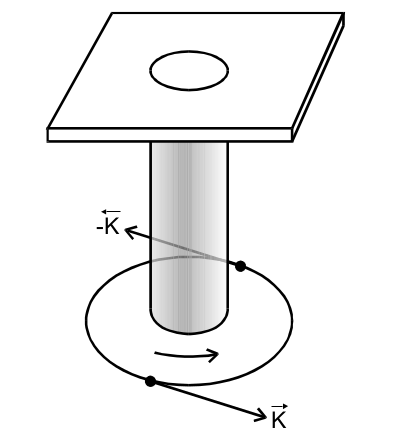
\includegraphics[height=6cm]{Drahttorsion.png}
  \caption{Torsion eines Drahtes.}
  \label{fig:Torsion}
\end{figure}

Dadurch greift ein Drehmoment $M$ am Draht an und die
Mantelflächen erfahren eine Scherung mit dem Winkel $\alpha$, sodass die
Stirnflächen um einen Winkel $\varphi$ phasenverschoben sind.
In Abbildung \ref{fig:TorsionMantel} sind diese Winkel und weitere Größen
eingezeichnet, die für den Zusammenhangs zwischen Drehmoment $M$
und Phasenwinkel $\varphi$ bedeutend sind.

\newpage

\begin{figure}
  \centering
  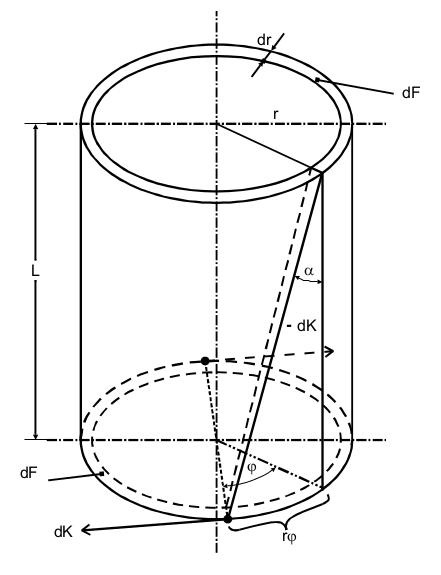
\includegraphics[height=9cm]{SkizzeFormel.png}
  \caption{Zusammenhang zwischen Drehmoment und Drillwinkel $\phi$.}
  \label{fig:TorsionMantel}
\end{figure}

Da das Drehmoment abhängig vom Radius ist, ergeben sich die infinitesimalen
Drehmomente durch Integration über die Mantelflächen mit der Gleichung

\begin{equation}
  \symup{d}M = r \cdot \tau \cdot \symup{d} F,
\end{equation}
wobei $\symup{d}F$ ein Mantelflächenelement ist.
Über das Hookesche Gesetz \eqref{eqn:Hooke}, die Formel zur Scherung eines
Körpers \eqref{eqn:Scherung} und die Winkelbeziehung

\begin{equation}
  \alpha = \frac{r\varphi}{L}
\end{equation}
folgt die proportionale Beziehung zwischen Drehmoment $M$, Phasenwinkel
$\varphi$ und Torsionsmodul $G$

\begin{equation}
  M = \int_{0}^{R} 2\pi \frac{G}{L} \varphi r^3 \symup{d}r = \frac{\pi}{2} G
  \frac{R^4}{L} \varphi.
  \label{eqn:tordDraht}
\end{equation}
Der Proportionalitätsfaktor

\begin{equation}
  D = \frac{\pi G R^4}{2L}
  \label{eqn:Richtgr}
\end{equation}
wird als Richtgröße des Zylinders bezeichnet.
Um nun zu einer dynamischen Messmethode zu gelangen, wird der Aufbau
um einen Körper mit dem Trägheitsmoment $\theta$ erweitert, der an das untere
Ende des Drahtes gehängt wird.
Wird der Draht mit dem Zusatzgewicht aus der Gleichgewichtslage ausgelenkt, so
führt das System harmonische ungedämpfte Drehschwingungen aus. In diesem
dynamischen Aufbau greifen sowohl das Drehmoment des tordierten Drahtes
\eqref{eqn:tordDraht}, als auch das der rotierenden Masse

\begin{equation}
  M_\text{T} = \theta \frac{\symup{d}^2\varphi}{\symup{d}t^2}
\end{equation}
an.
Die daraus resultierende Differentialgleichung

\begin{equation}
  D \varphi + \theta \frac{\symup{d}^2\varphi}{\symup{d}t^2} = 0
\end{equation}
kann mit dem Ansatz

\begin{equation}
  \varphi(t) = \varphi_0 \cos \Bigl(\frac{2\pi}{T}t\Bigr)
\end{equation}
mit der Auslenkung $\varphi_0$ gelöst werden.
Es folgt die Periodendauer der Schwingung

\begin{equation}
  T = 2\pi \sqrt{\frac{\theta}{D}}
  \label{eqn:Periodendauer}
\end{equation}
Da die Periodendauer $T$ sehr genau messbar ist kann über die
Gleichung zur Richtgröße des Zylinders \eqref{eqn:Richtgr} und dem
Trägheitsmoment des Körpers aus der Formel \eqref{eqn:Periodendauer} der
Torsionsmodul $G$ bestimmt werden.
Das Trägheitsmoment $\theta$ berechnet sich über die Formel

\begin{equation}
  \theta = \int_{\partial V}^{} \rho(\vec{r}) r_\perp^2 \symup{d}V
\end{equation}
mit der Massendichte $\rho$, dem Abstand zur Rotationsachse $r_\perp$ und dem
Volumenelement $\symup{d}V$.
Für die im folgenden Versuch verwendete Kugel mit konstanter Massendichte
folgt dann
\begin{equation}
  \theta_\text{k} = \frac{2}{5} m_\text{k} R_\text{k}^2
\end{equation}
mit der Kugelmasse $m_\text{k}$ und dem Kugelradius $R_\text{k}$.
Die entgültige Gleichung für den Torsionsmodul $G$ lautet dann

\begin{equation}
  G = \frac{16}{5} \pi \frac{m_\text{k}R_\text{k}^2 L}{T^2 R^4}.
\end{equation}


\subsection{Magnetisches Moment}

gauß bei rlc gedämpfte schwingung

\cite{sample}
